\documentclass{standalone} 

\usepackage{pgfplots}
    \pgfplotsset{compat=1.16}

\begin{document}
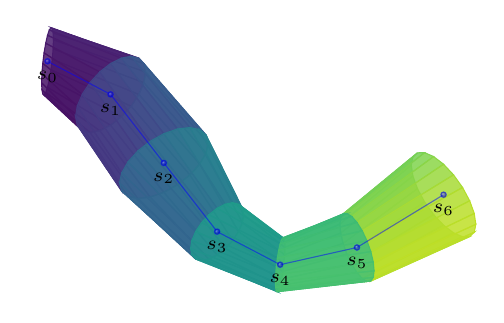
\begin{tikzpicture}
    \begin{axis}[
    view={10}{40},
    hide axis,
    axis equal,
    axis equal image,
    ]
    % \draw[thin] (axis cs: 0,0,0) -- (axis cs: 0.5,0,0);
    % \draw[thin] (axis cs: 0,0,0) -- (axis cs: 0,0.5,0);
    % \draw[thin] (axis cs: 0,0,0) -- (axis cs: 0,0,0.5);
    \def\A{(0.25+0.05*sin(x*420))}
    \def\B{1}
    \def\PI{3.14159265359}
    \addplot3[
        surf,
        % shader=interp,
        shader=flat,
        domain=0:1,
        samples=7,
        samples y=21,
        y domain=0:360,
        colormap/viridis,
        % opacity=0.0,
        fill opacity=0.85,
        point meta=x,
        z buffer=sort,
    ]
    ({(\B*\PI*x + sin(\B*x*270)*sin(y)*\A)*100}, {(cos(\B*x*270) + sin(y)*\A)*100}, {cos(y)*\A*100});
    % 
    % \addplot3[
    %     mesh,
    %     % surf,
    %     % shader=flat,
    %     domain=0:1,
    %     samples=7,
    %     samples y=7,
    %     y domain=0:360,
    %     colormap/viridis,
    %     % opacity=0.0,
    %     % fill opacity=1,
    %     point meta=x,
    %     z buffer=sort,
    % ]
    % ({\B*\PI*x + sin(\B*x*270)*sin(y)*\A}, {cos(\B*x*270) + sin(y)*\A}, {cos(y)*\A});
    % 
    % \addplot3[
    %     surf,
    %     shader=flat,
    %     domain=0:1,
    %     samples=7,
    %     samples y=7,
    %     y domain=0:360,
    %     scatter/use mapped color={ball color=blue!50!black},
    %     scatter,
    %     only marks,
    %     mark=ball,
    %     mark size=0.75pt,
    % ]
    % ({\B*\PI*x + sin(\B*x*270)*sin(y)*\A}, {cos(\B*x*270) + sin(y)*\A}, {cos(y)*\A});
    % 
    \addplot3[
        domain=0:1,
        samples=7,
        samples y=0,
        draw=blue,
        opacity=0.5,
        mark=ball,
        mark size=1.0pt,
        % nodes near coords={$p_\coordindex$},
        % nodes near coords align={below},
        % every node near coord/.append style={font=\small},
    ]
    ({\B*\PI*x*100}, {cos(\B*x*270)*100}, {0});
    \addplot3[
        domain=0:1,
        samples=7,
        samples y=0,
        only marks,
        % draw=blue,
        % opacity=0.5,
        % mark=ball,
        % mark size=1.0pt,
        nodes near coords={$\scriptstyle s_{\scriptscriptstyle\coordindex}$},
        nodes near coords align={below},
        % every node near coord/.append style={font=\small},
    ]
    ({\B*\PI*x*100}, {cos(\B*x*270)*100}, {0});
    % 
    % \addplot[only marks,mark=*,mark options={scale=0.5, fill=red},text mark as node=true,point meta=explicit symbolic,nodes near coords] coordinates { (0,0) [A]   (2,4) [B]};
    % 
    \end{axis}
\end{tikzpicture}
\end{document}